\subsection{Rosemary}

\paragraph{Testing the data model's flexibility}
\begin{figure}[!b]
	\centering
	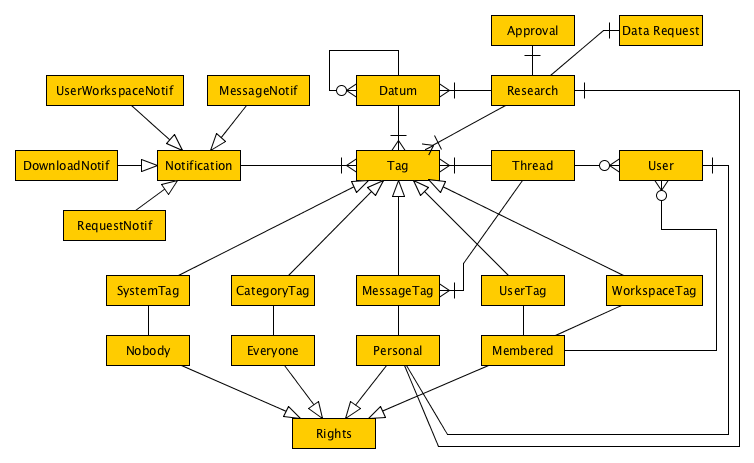
\includegraphics[width=1.0\linewidth]{images/datamodel-adapted}
	\caption{
		Rosemary data model as implemented.
		Describes workspace, tagging, datum, notification, and research models.
		The original data model can be found in figure \ref{fig:reuse-rosemary-dm}.
		Differences between the implemented model and the original model are shown in blue.
	}
	\label{fig:implementation-rosemary-dm}
\end{figure}

As mentioned earlier in section \ref{reuse-rosemary} alterations had to be made to the original Rosemary data model.
These can be divided into additions in the form of new objects and changes to already existing objects.

The only existing object needing changes is the {\tt WorkspaceTag}.
This tag is used to tell the system what subsets of data exist, where each subset is made up of one or more {\tt Datum}s (\ie{} each {\tt Datum} tagged with a certain workspace tag belongs in the subset).
Each tag also has an owner and members, all the users in this set has access to the data in the workspace.

The original Rosemary implementation does not differentiate between different \emph{types} of workspaces. 
The \ivfsystem{} has a \emph{master} workspace containing \emph{all} the raw data from every clinic, it has clinic workspaces containing data specific to a clinic, and it has request workspaces containing data for a specific request.
This is reflected by adding a workspace type field to the {\tt WorkspaceTag} object.

Requests contain a limited set of data items (headers), the \emph{master} dataset contains all the available headers.
To restrict the headers a researcher can view in his or her request workspace a visibility field was added to the {\tt WorkspaceTag}.
This field contains a set of the accessible headers for a workspace, the system can then filters this data from the \emph{master} dataset before outputting the result to the user.

Next to these two (minor) changes five new data objects were added to the data model.
These are: {\tt Research}, {\tt Approval}, {\tt Data Request}, {\tt DownloadNotif}, {\tt RequestNotif}.
The two notification objects are used to determine how information is displayed in the front-end they both inherit from the {\tt Notification} object.
This means that the methods used to extract information are standardised and these two notification objects can directly be used in the system without further need for customisation.

The other three objects are related to each other, each {\tt Research} contains an {\tt Approval} object and an {\tt Data Request} object.
These related objects are used to capture data regarding the request progress.
Where the {\tt Data Request} contains the requested headers and the {\tt Datum}s these relate to in the \emph{master} dataset.
And the {\tt Approval} keeps record of the committee users that need to give permissions and what votes were already cast.
Lastly, the {\tt Research} object is used to capture information used to base a voting decision on, \eg{} research question, study description.

\paragraph{Back-end and front-end}
In Rosemary the back-end provides an RESTful API which the front-end can communicate with, meaning that the back-end is completely disjointed from the front-end.
Communication is done with JSON\footnote{http://json.org/}, which leaves options open for a complete rebuild of the front-end without having to touch the back-end.
For the \ivfsystem{} the existing back and front-end were both reused.

Starting with the back-end, some structural changes were made.
Firstly, classes and methods that were used for submission and application handling were removed.
Also the data import function was removed, however this might find a place in a later prototype of the \ivfsystem{} when incremental updating of data is used.
Then, each of the objects from the data model are implemented in the back-end through a class.
For each of the new objects a class was created with the necessary methods to store and retrieve data in them.

The most notable changes to existing code were in the data handling and security classes.
Rosemary already supports basic user handling where a user creates an account and access to the system is restricted based on this.
However the system needed user roles for a fine grated control of access to the system.
To execute this control the system requires these roles to be read and acted upon.
This is reflected in the security class which now supplies this information.

Data handling had to be changed in the sense that most of the time {\tt Datum}s would be retrieved with only a small selection of the available headers.
All the read methods in the data class have been adapted to restrict access.
This makes for easy access of data from the front-end, it just provides the back-end with a request for a workspace with a certain user.
The back-end then filters data based on this and returns the restricted dataset.

Design of front-end was done on an educated guess base.
There was no time available for a user-centred design approach where prototypes are iterated until the best design solution is achieved.
The existing layout was mostly left in place, pages related to surplus functions (submission and application handling) were removed.
For each of the new functions pages were created where necessary.

To the architecture of the front-end no changes were made.
The implementation of back-end communication and security was sufficient for a successful implementation of a prototype.